\documentclass[12pt, a4paper]{article}

\usepackage[utf8]{inputenc}
\usepackage{lmodern}
%\usepackage{fourier}
\usepackage{setspace}
	\singlespacing

\usepackage[frenchb]{babel}
\usepackage{xspace}
\usepackage[margin= 2.5cm]{geometry}
\pagestyle{plain}
\renewcommand{\thefootnote}{\fnsymbol{footnote}}

\usepackage{tikz}
	\usetikzlibrary{shapes}
\usepackage{graphicx}
	\graphicspath{{img/}}

\usepackage{varioref}
	\renewcommand{\reftextbefore}{page précédente}
	\renewcommand{\reftextfacebefore}{page ci-contre}
	\renewcommand{\reftextafter}{page suivante}
	\renewcommand{\reftextfaceafter}{page ci-contre}
	\renewcommand{\reftextcurrent}{}

\usepackage{amsmath, amsfonts}
\everymath{\displaystyle}


\newcommand{\espace}{\vspace{.8cm}}
\newcommand{\pg}{

}

%% REMPLIR
\usepackage[colorlinks=true, allcolors=blue, pdfborder={0 0 0}]{hyperref}
	\hypersetup{
		pdftitle={Super Original},
		pdfsubject={Rapport Super Original},
		pdfkeywords={Super Original, IARISS, rapport},
		pdfauthor={IARISS Team}
	}
\title{Défi Super Original}
\newcommand{\authors}{Jérémy, Florent}

%
\begin{document}

\author{
\includegraphics{../_img/iariss_team.png} \\ {\sffamily \href{http://iarissteam.me}{iarissteam.me}}}
\date{\today}

\maketitle{}

{\sffamily DESCRIPTION A FAIRE} 

\espace{}
\section{Le Projet : compte à rebours, live, timelapse, tumblr}
 
- Nous avons procédé à la mise en place d'un compte à rebours avant le début de la nuit de l'info (d'abord avec une actualisation hebdomadaire, puis ensuite un vrai décompte à partir de H-1, seconde par seconde), puis avant la fin de la Nuit de l'Info (en fond de notre \href{http://iarissteam.me/}{portail}).

- Un live a été diffusé (\href{http://live.iarissteam.me/}{http://live.iarissteam.me/}) dès le début de la nuit, et pendant toute la durée de celle-ci. Cela a impliqué la réservation préalable d'un nom de domaine.

- Une seconde webcam a été mis ene place en parallèle dans le but de réaliser un timelapse (disponible \href{ici}{ici}). A partir de 14h et jusqu'à la fin de la nuit, une photo a été prise toute les secondes. Toutes ces images ont ensuite été résumé dans une vidéo résumant la Nuit de l'Info, en accéléré.

- Enfin, un tumblr \href{http://lesjoiesdelanuit.tumblr.com/}{Les Joies de la Nuit} (inspiré de \href{http://lesjoiesducode.tumblr.com/}{Les joies du Code}), avec tweet automatique pour chaque nouvel article posté. Ce tumblr a été alimenté touteau long de la nuit, par des articles préparées à l'avance, mais aussi en \og{}live\fg{}, en fonction des différents évènements arrivés au cours de la nuit.

\espace{}
\section{Communication : }
Toute la nuit, une équipe de trois personnes à temps partiel s’est relayée pour réagir et interagir sur \href{https://twitter.com/}{Twitter} et valoriser le live et le décompte. En parallèle les nouveaux posts sur \href{http://lesjoiesdelanuit.tumblr.com/}{Les Joies de la Nuit} sont automatiquement tweetés. Pour chaque tweet, le hashtag \#nuitinfo est utilisé.
En outre, le principe du live permet de tweeter toute action se déroulant dans la salle, tel que les visites inopportunes ou autre, en revoyant en plus sur le live par un lien (15 viewers en moyenne sur la nuit).

\espace{}
\section{Exemple d'action et quelques photos : }
\href{https://twitter.com/}{Twitter}
\espace{}
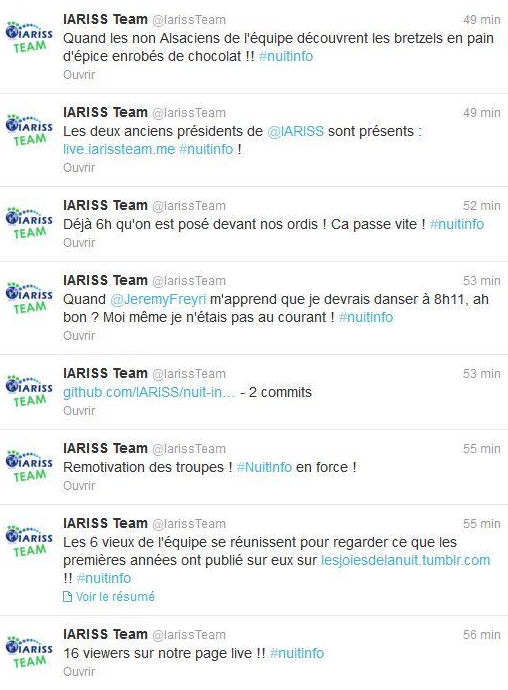
\includegraphics[width=.9\textwidth, keepaspectratio=true]{img/twitter.png}
\espace{}

\href{http://iarissteam.me/}{Notre portail, avec le compte à rebours}
\espace{}
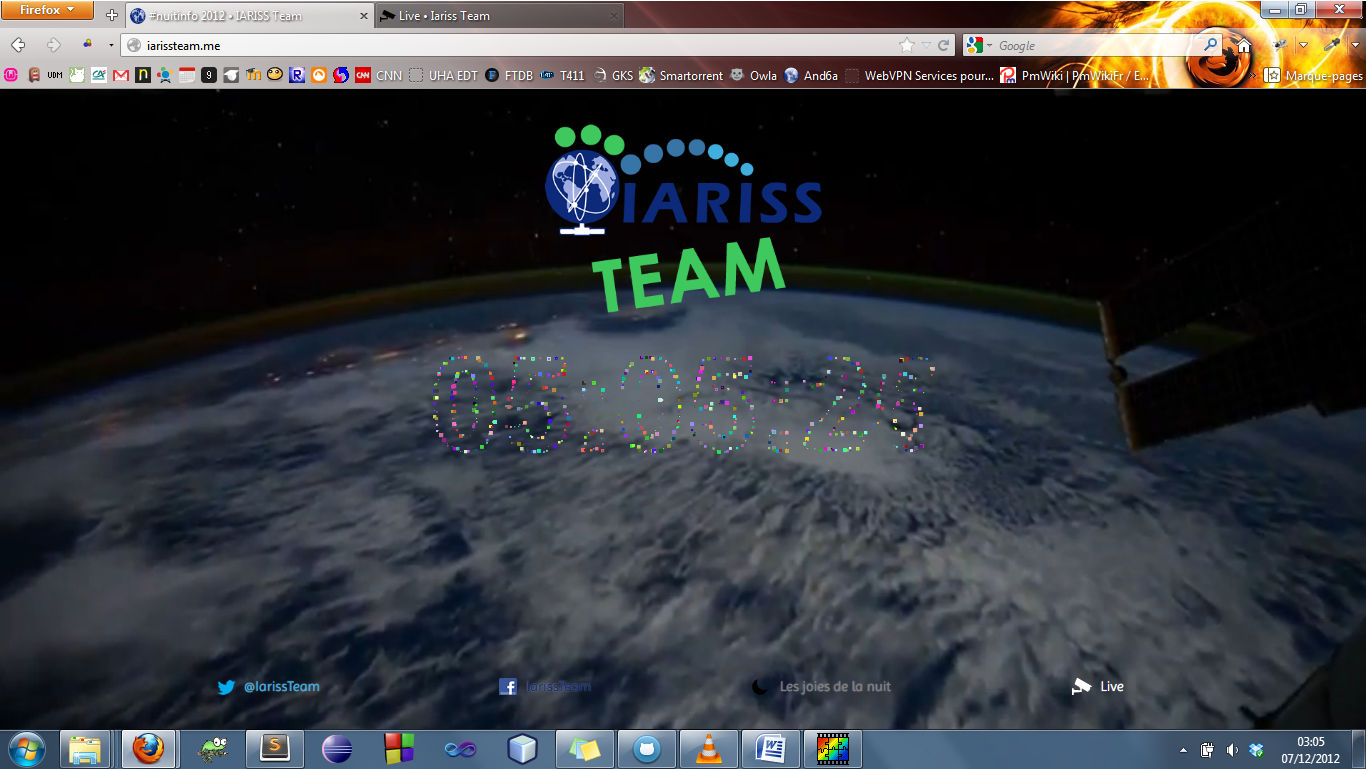
\includegraphics[width=.9\textwidth, keepaspectratio=true]{img/portail.png}
\espace{}

\href{http://live.iarissteam.me/}{Notre live}
\espace{}
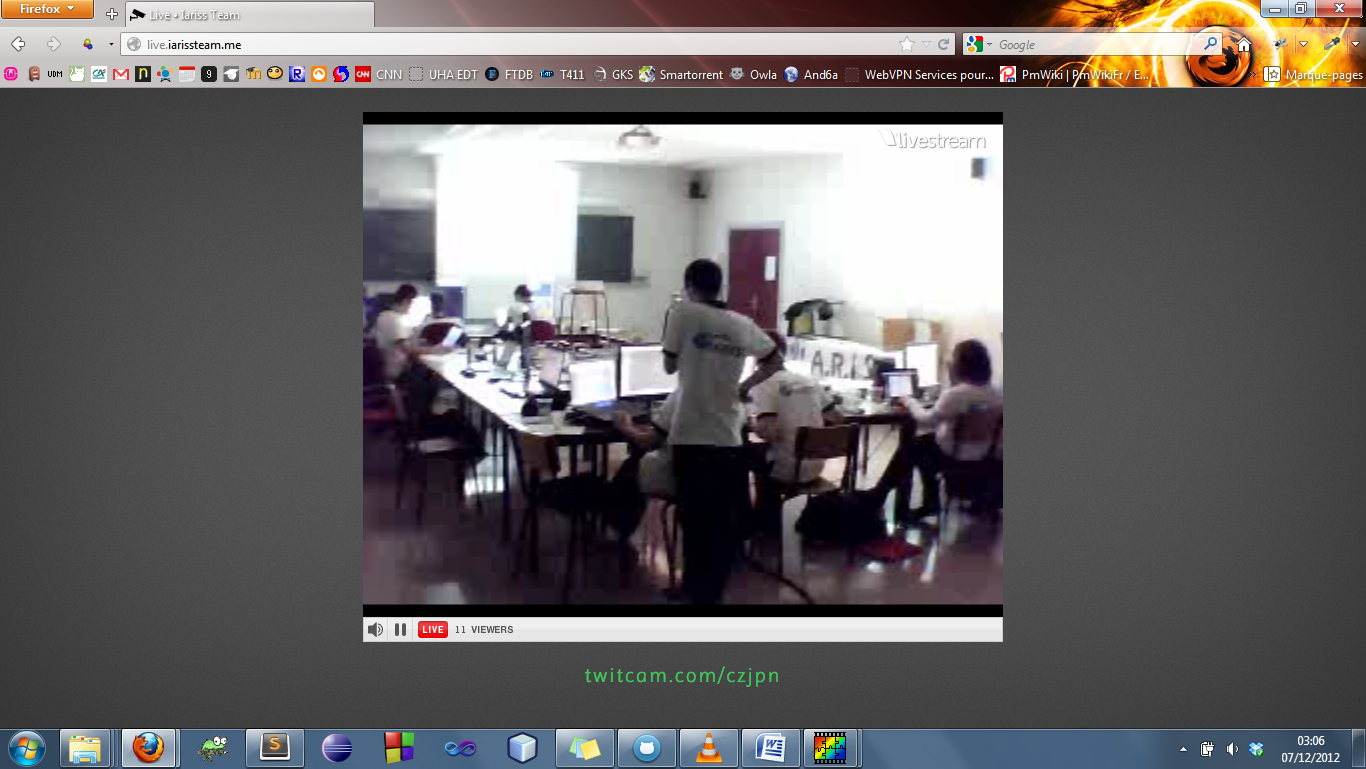
\includegraphics[width=.9\textwidth, keepaspectratio=true]{img/live.png}
\espace{}

Une de nos installations : un dualscreen avec des vidéos projecteurs, permettant d'afficher simultanéement Twitter et notre portail ou notre live par exemple.
\espace{}
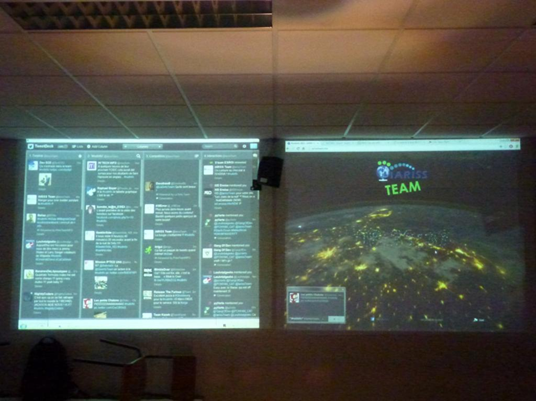
\includegraphics[width=.9\textwidth, keepaspectratio=true]{img/photo1.png}
\espace{}
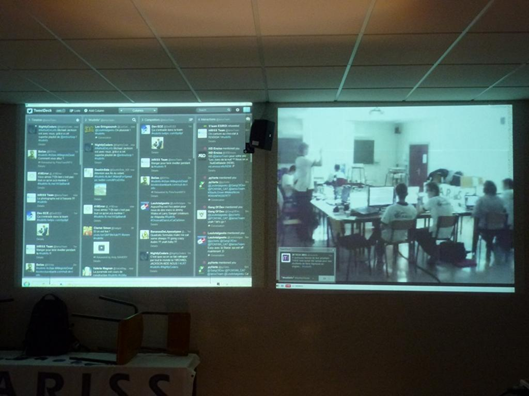
\includegraphics[width=.9\textwidth, keepaspectratio=true]{img/photo2.png}
\espace{}


%\espace{}
%\begin{figure}[h]
%	\begin{center}
%	\end{center}
%	\caption{\label{fig-} Légende}
%\end{figure}

\espace\vfill{}
Ce document a été rédigé en \LaTeX{} par \authors{} pour IarissTeam avec quelques tasses de café et beaucoup de bonne humeur.

Contactez-nous à \href{mailto:nuitinfo@iariss.com}{nuitinfo@iariss.com} pour tout renseignement supplémentaire !

\end{document}